\documentclass{article}

\usepackage[usenames]{color}
\usepackage{graphicx}
\usepackage{amsmath}
\usepackage{amsfonts}
\usepackage{amssymb}
\usepackage{mathrsfs}
\usepackage{bm}
\usepackage{verbatim}
\usepackage{cancel}

\begin{document}

\begin{figure}[htbp]

%\centering
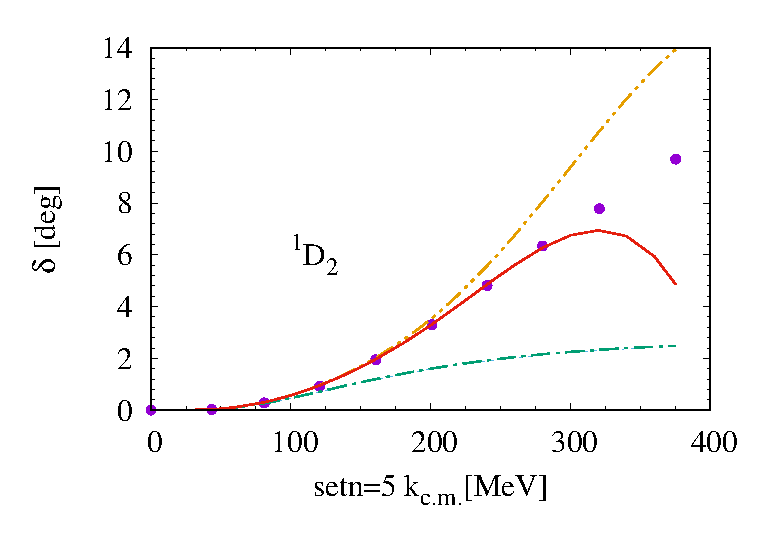
\includegraphics[width=0.5\textwidth]{5_1d2.eps}
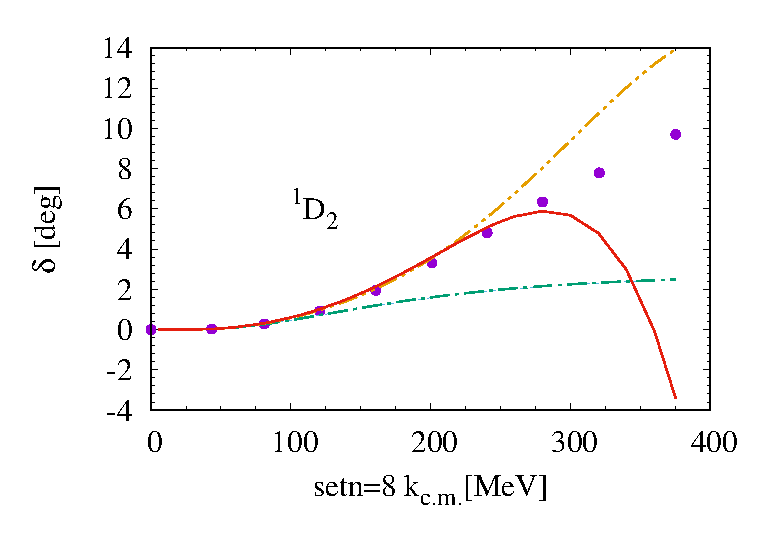
\includegraphics[width=0.5\textwidth]{8_1d2.eps}
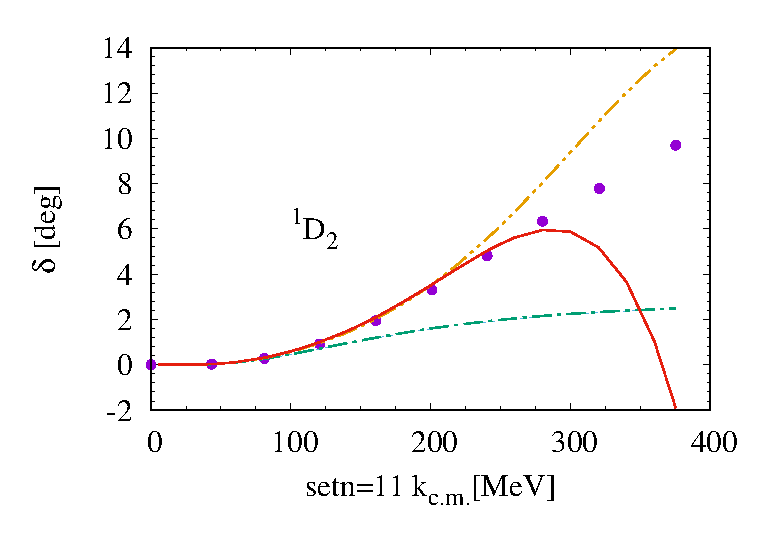
\includegraphics[width=0.5\textwidth]{11_1d2.eps}
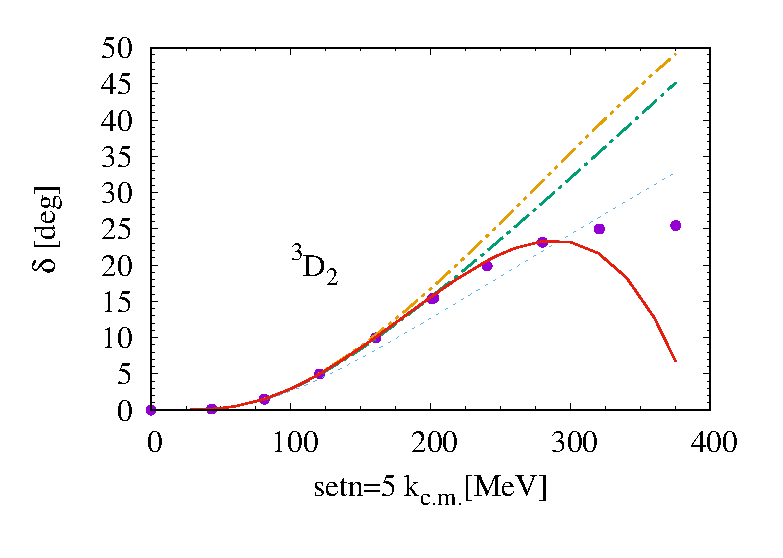
\includegraphics[width=0.5\textwidth]{5_3d2.eps}
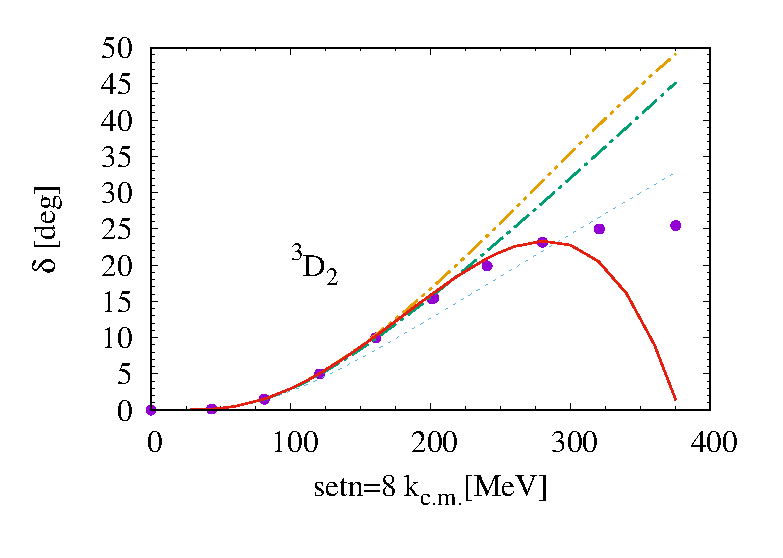
\includegraphics[width=0.5\textwidth]{8_3d2.eps}
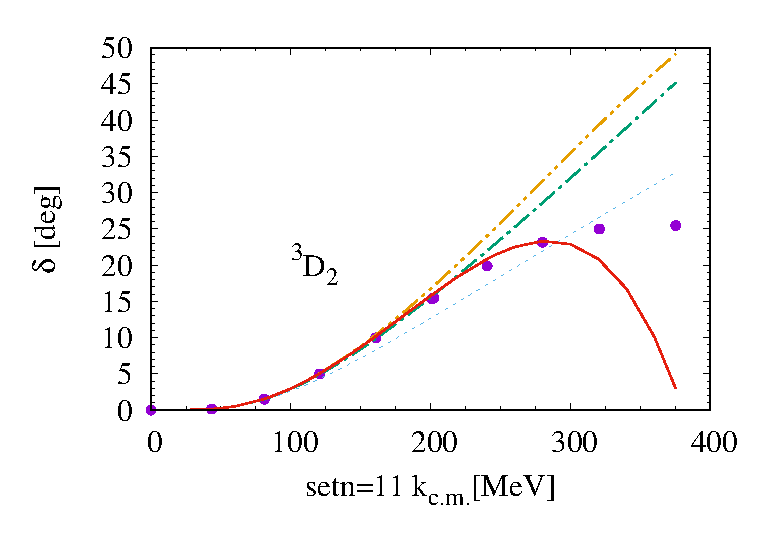
\includegraphics[width=0.5\textwidth]{11_3d2.eps}
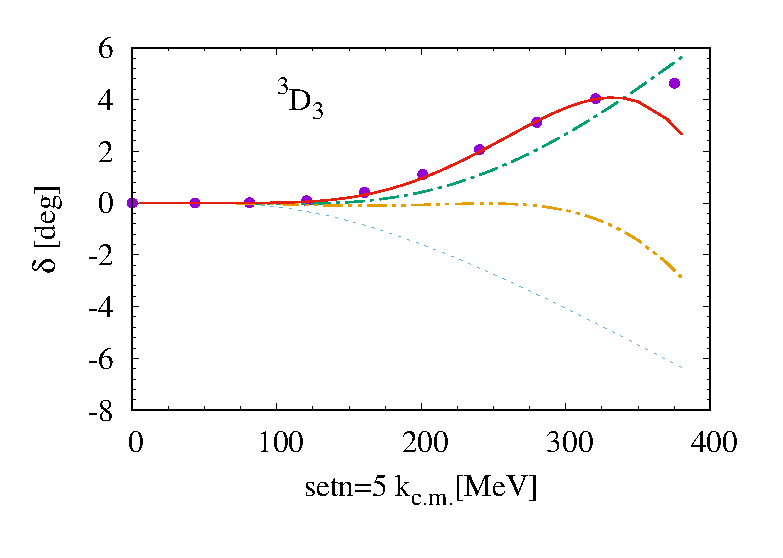
\includegraphics[width=0.5\textwidth]{5_3d3.eps}
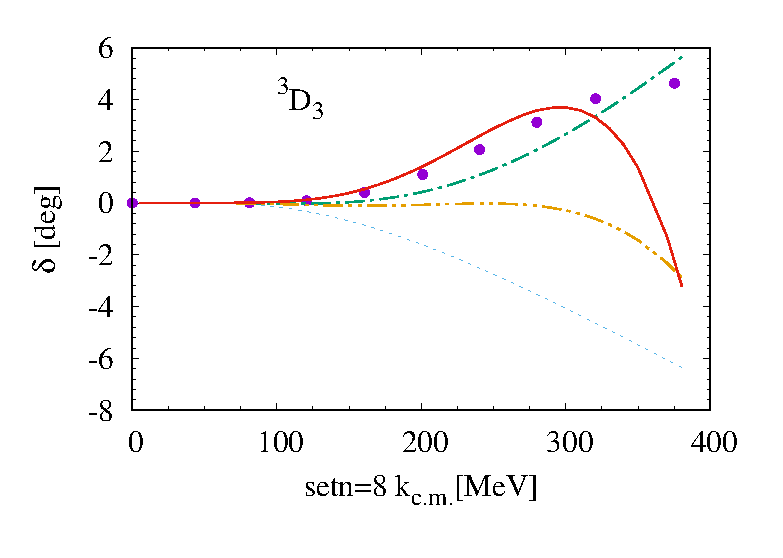
\includegraphics[width=0.5\textwidth]{8_3d3.eps}
\end{figure}
%\newpage
%\pagebreak[2]
\begin{figure}[htbp]
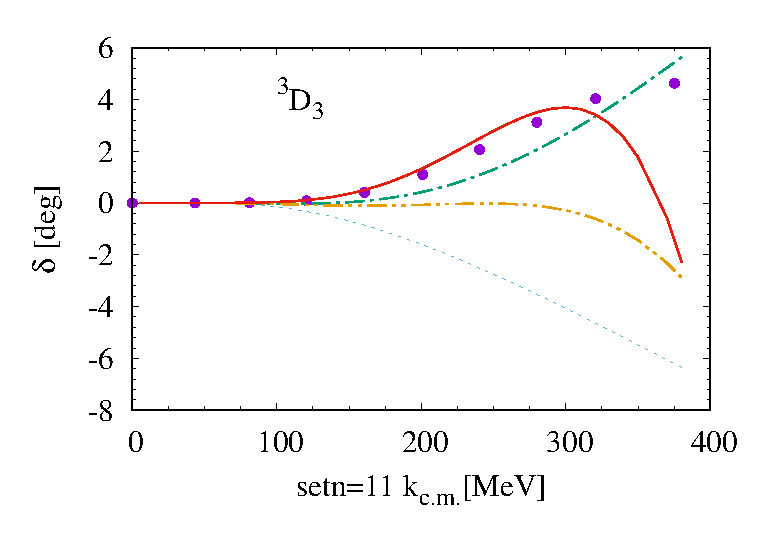
\includegraphics[width=0.5\textwidth]{11_3d3.eps}
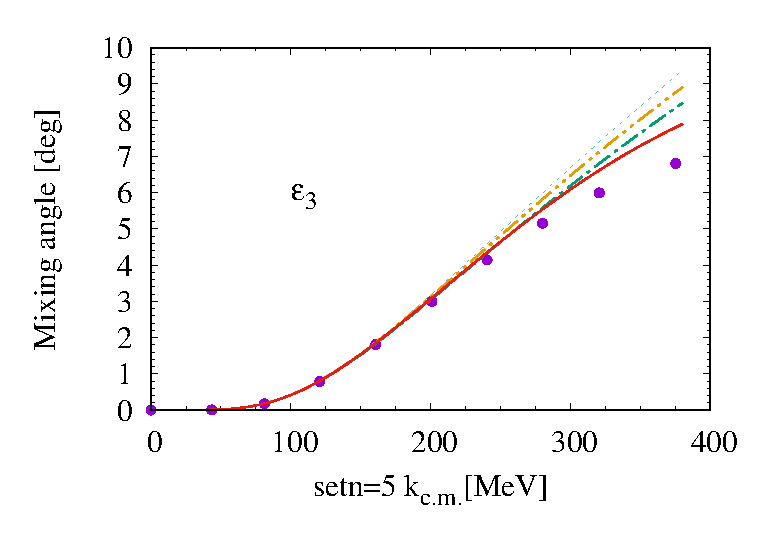
\includegraphics[width=0.5\textwidth]{5_e3.eps}
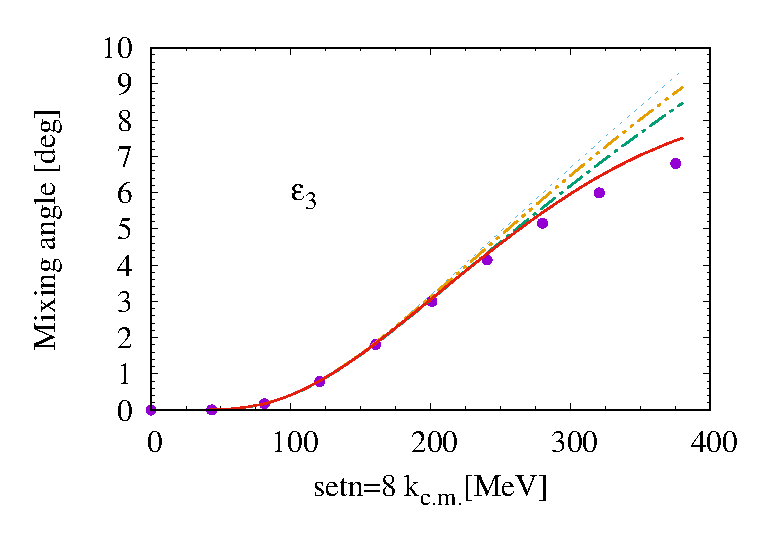
\includegraphics[width=0.5\textwidth]{8_e3.eps}
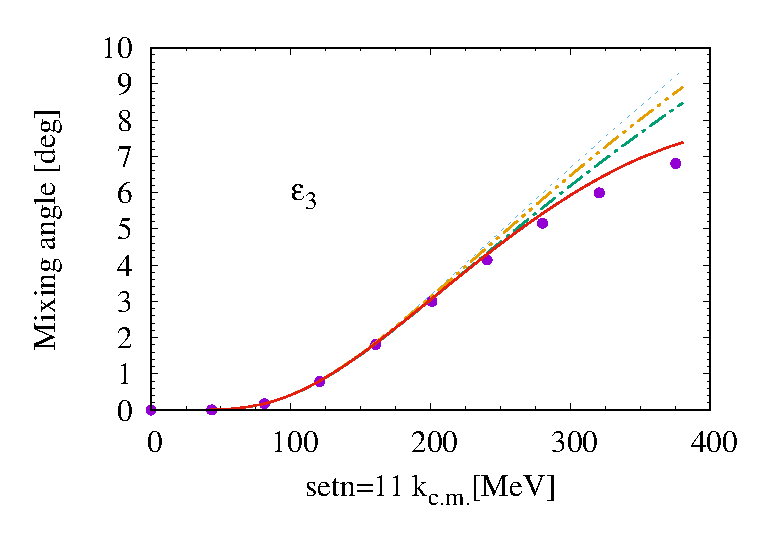
\includegraphics[width=0.5\textwidth]{11_e3.eps}
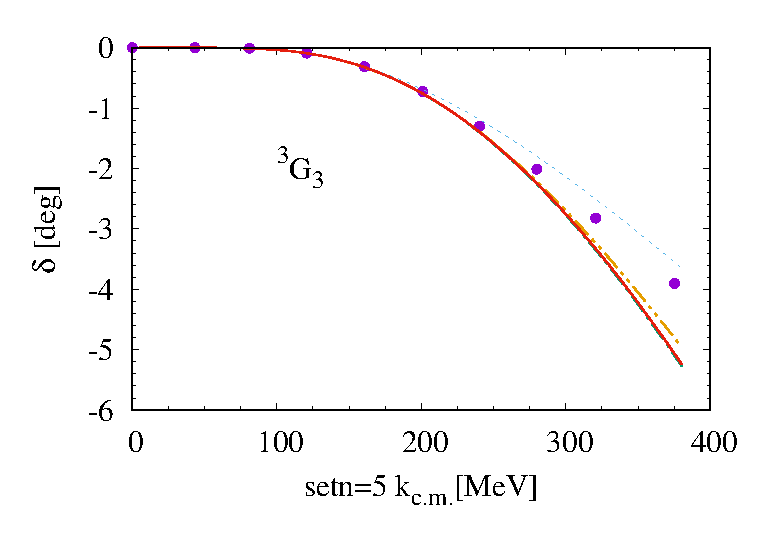
\includegraphics[width=0.5\textwidth]{5_3g3.eps}
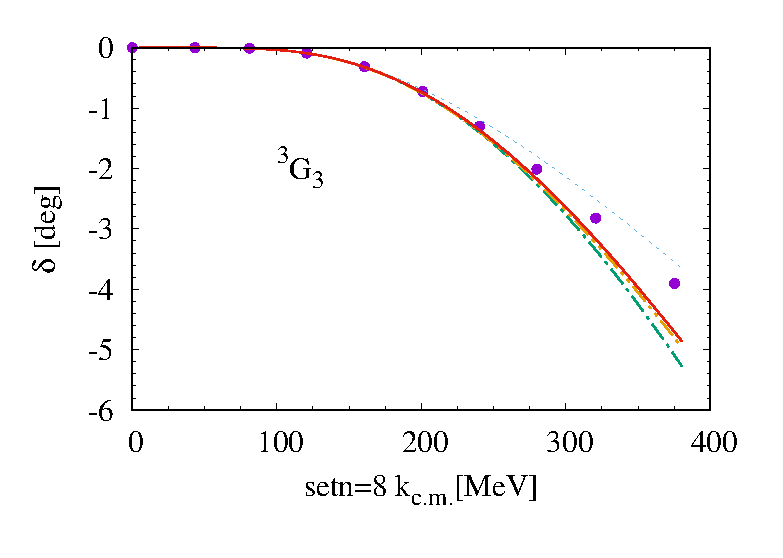
\includegraphics[width=0.5\textwidth]{8_3g3.eps}
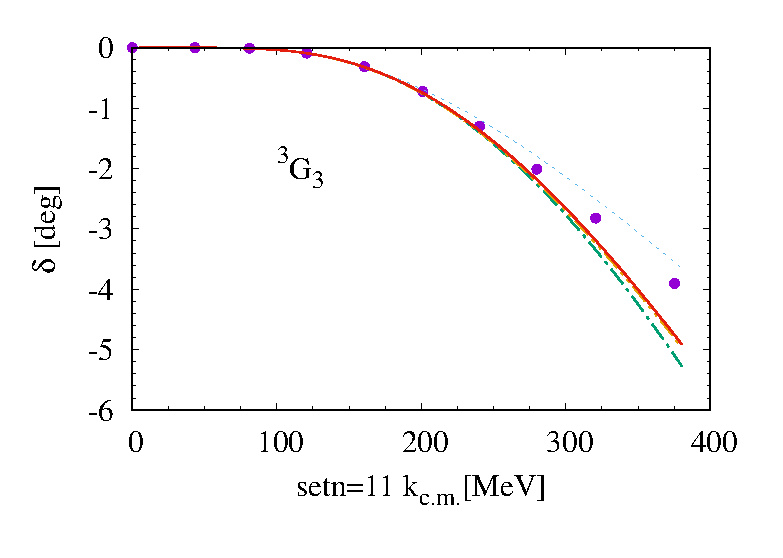
\includegraphics[width=0.5\textwidth]{11_3g3.eps}
\caption{The bule, green, orange, and red lines correspond respectively to NLO, N$^2$LO, N$^3$LO, and N$^4$LO. }
\end{figure}

\end{document}